\documentclass[a4paper]{article}
\usepackage[left=2cm, right=2cm, top=2cm]{geometry}
\usepackage{tikz}
\usepackage{algorithm}
\usepackage{graphicx}
\usepackage{amsmath}
\usepackage{float}
\usepackage{listings}

\def\code#1{\texttt{#1}}
\lstset{
frame=single
}

\author{Kevin Mambu}
\title{UE-VLSI2 TP : Cadence RTL Compiler \\ Kévin Mambu, Nicolas Phan}
\begin{document}
\maketitle

\section{Set the environment}

\lstinputlisting[language=bash]{../set_env.sh}


\section{Load the libraries}

{\it n.b: all the libraries are located at} \code{/users/enseig/tuna/ue-vlsi2/techno}.

Two types of cell libraries are available:
\code{\_Best.lib} and \code{\_Worst.lib}. The difference between these libraries
lies in the timing arcs of their cells : while the Best Library contains Best-Case timings,
the Worst Library contains the Worst-Case equivalents. Each timing arcs are estimated via
different PVT parameters (\textbf{Process - Voltage - Temperature}). These parameters can be
found in the headers of each library.

\lstinputlisting{cmos_120nm_core_Worst_header.txt}
\begin{center}
  \it{PVT specifications for cmos\_120nm\_core\_Worst}
\end{center}

\newpage

\lstinputlisting{cmos_120nm_core_Best_header.txt}
\begin{center}
  \it{PVT specifications for cmos\_120nm\_core\_Best}
\end{center}

In order to synthesize the RTL description, we will use cmos\_120nm\_core\_Worst.lib.
This library contains all the generic cells we will need, and with Worst-Case timings
in order to thoroughly stress the longest combinational paths.

A practical example of difference in timing arcs between this library and its \_Best
equivalent can be seen when evaluating the ND2AHS cell, a "2 Input NAND w\/ A Input
Inverted and 1x Drive".

\begin{center}
  \hspace{6em}
  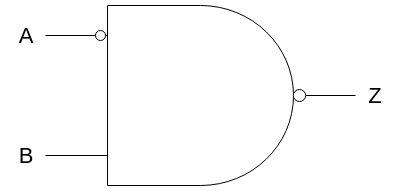
\includegraphics[width=10cm]{./nd2ahs.png} \newline
  \it{Gate-level schematic of the ND2AHS cell}
\end{center}
% TODO : mettre un comparatif WC/BC
%        demander à l'homme-sirène s'il faut faire le schéma symbolique de la
%        cellule?
\section{Load the design}

\section{Elaborate}

The eaboration process does not differ from the Synthesis per se. The elaboration step
is the conversion of the RTL description to a model where every instance object (signal,
process, arrays, etc) is converted into a component (adder, multiplexer, register, etc).
This step is part of the Synthesis process.

\section{Check design}

\section{Synthesis}

\section{Reset}
There are two reset signals in the design :
\begin{enumerate}
  \item RESET\_N is the external reset signal. Its whereabouts are not bound by any timing
  constraints and its value can change at any time, as the signal comes from outside the
  design through an interface pad. This is an asynchronous reset signal.
  \item RESET\_RX is the internal reset of the design. This one is synchronous as its
  value is refreshed at every rising edge of the clock.
\end{enumerate}

First we should precise that while the activation of the reset ($0 \rightarrow 1$) is asynchronous,
its deactivation ($1 \rightarrow 0$) has to be synchronized with the clock. The design itself is
synchronous and the transition from the reset state to the initialization state is synchronous as
well. This is the utility of the RESET\_RX register.

Still the external reset is a potential hazard for the design, as it comes from the outside. We cannot
simply assume that the propagation of the signal was flawless and must consider that it may have
had issues on its way:
\begin{enumerate}
  \item The external reset may come from a different clock domain. In that case, the signal would have
  been synchronous in its previous clock domain but would appear asynchronous when entering the design.
  \item The external reset may be already asynchronous.
\end{enumerate}
In any case, the external reset signal may arrive in the design without respecting constraints relative
to the setup time of its imminent receptor (a flip-flop, for example).
All these possibilities may bring the value of the signal to a metastable state, where its value is
indetermined before setting itself to a non-deterministic, but stable value. The probability of such an
event is rare but not impossible, and the propagation of such a signal may bring the design to a
non-deterministic state, ruining the function of the design.

A Reset Synchronizer is a component with an asynchronous signal as input and an asynchronous signal as
output. In order to prevent the propagation of a metastable value, the reset synchronizer uses the
probabilistic properties of meta-stability : a meta-stable state is always short-lived, and while we
cannot predict the end of a meta-stable state, we know for sure that it won't perdure long before
setting itself for good.

Let $\epsilon$ be the probability for an asynchronous reset to bring a flip-flop to a meta-stable state.
For $n$ being the number of flip-flops on a given datapath, the probability of meta-stability being propagated
through the datapath is $\epsilon^n$. This property makes so that a Reset Synchronizer slims down the
probability of the propagation of meta-stability to virtually none.

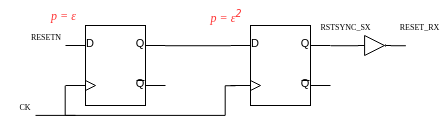
\includegraphics[width=15cm]{./reset_synchronizer.png}
\begin{center}
  {\it Schematic of a 2-register Reset Synchronizer. In red are the corresponding probabilities of a
  propagation of meta-stability.}
\end{center}

This model was implemented to the design. The verification of the functionnality was done using GHDL.
\begin{center}
  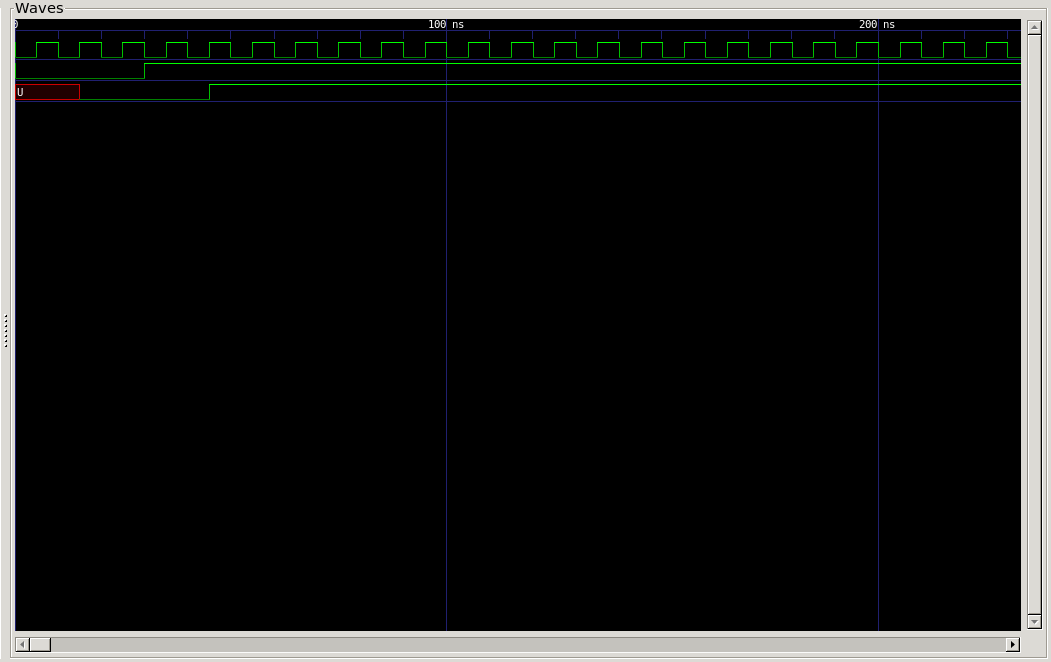
\includegraphics[width=15cm]{./reset_sync_waveform.png}\\
  {\it Waveform of the Reset Synchronizer using GTKWave}
\end{center}

\lstinputlisting[language=vhdl,caption={RTL description of the Reset Synchronizer}]{../reset_synchronizer.vhd}

\newpage

\section{Reporting}
From the area report, the design is composed of 13878 cells, and has a surface of 220290 square cells.

The timing report gives the longest datapath of our design. We can see that its start point is the I\_RI register
and its end point the NEXTPC\_RD register. The total delay of this datapath is 11.538ns.
The maximum frequency, evaluated only from this timing report, equals $\dfrac{1}{11538\times10^{-15}}$ Hz, or
approximately 86.670 GHz.
The timing slack of a connection is the difference between its required time and its arrival time. In our design
the timing slack is UNCONSTRAINED because no timing constraints have been specified yet. Because of this omission,
no clock signal are emitted on the design.

When anayzing the lint timing report, we can see the following warning catergories :
\begin{enumerate}
  \item Generated clocks without clock waveform
  \item Inputs without clocked external delays
  \item Outputs without clocked external delays
  \item Inputs without external driver/transition
  \item Outputs without external load
\end{enumerate}

\section{Constraints}
\subsection{Reg-To-Reg}
The clock constraint removed the "Generated clocks without clock waveform" issue.

\subsection{Input-To-Reg}
Let us consider the inputs for the CLOCK domain takes 1.2 nanoseconds to come. Since the clock period in the
CLOCK domain is 2 ns (from the addition to our .sdc file in the previous question), it means the arrival time
if its signal is 1 ns, for the falling as well as the rising edge. This means that our inputs will always be
late to the setup time limit by 0.2 nanoseconds and no inputs will actually be saved in our registers.

\begin{center}
  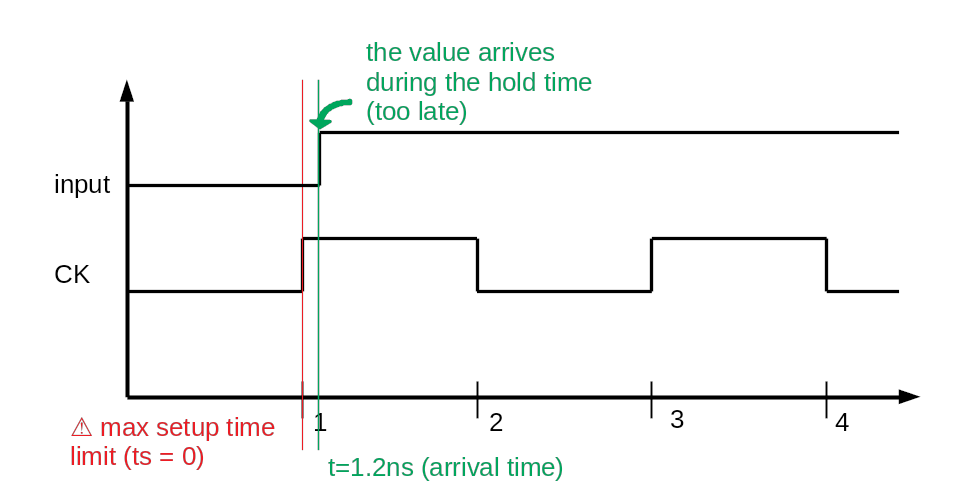
\includegraphics[width=14cm]{./timing_problem.png}
\end{center}

Let us actually specify this input delay to our .sdc file and check what the timing report tells us.
We can see that we do not have any more "Inputs without clocked external delays".

\subsection{Reg-To-Output}
We want to constraint the outputs of our design to a delay of 1.2 nanoseconds. After adding this to our sdc file,
we can see in our timing report that all our inputs and outputs have delays specified. Unfortunately, when we read
the entire timing report we can see, as expected, that there are timing violations.

This time, the worst path starts from the RD\_RE register and ends at D\_SYNC. The total delay is 12.542 nanoseconds,
which is really long. This is due to the definition of our inputs and outputs delays. Our clock definition impose a
capture time of 2 ns, which means our critical path, with our specified in/out delays, is too long for our clock
frequency. The timing slack is of -10.542 nanoseconds.

\section{Report timing}


\end{document}
